%%%%%%%%%%%%%%%%%%%%%%%%%%%%%%%%%%%%%%%%%%%%%%%%%%%%%%%%%%%% 
% This is the official template for theses and seminar papers from the Chair for Information Systems for Sustainable Society (IS3) at the University of Cologne

%
%PREAMBLE
%%%%%%%%%%%%%%%%%%%%%%%%%%%%%%%%%%%%%%%%%%%%%%%%%%%%%%%%%%%%%

\documentclass[a4paper, oneside, 12pt]{article}
\usepackage[utf8]{inputenc}
\usepackage[T1]{fontenc}
\usepackage{graphicx}
\usepackage{longtable}
\usepackage{hyperref}
\usepackage{caption}
\usepackage{amssymb}
\usepackage{amsmath}
\usepackage{todonotes}

% set margins for double-sided printing
\usepackage[left=2.5cm, right=2.5cm, top=2.5cm, bottom=2.5cm, bindingoffset=1.5cm, head=15pt]{geometry} 
\usepackage{setspace}
\onehalfspacing
% set headers
\usepackage{fancyhdr}
\pagestyle{fancy}
\fancyhead{}
\fancyfoot{}
\fancyhead[L,RO]{\textsl{\leftmark}}
\fancyhead[R,LO]{\thesisauthor}
\fancyfoot[C]{\thepage}
\renewcommand{\headrulewidth}{0.4pt}
\renewcommand{\footrulewidth}{0pt}

% set APA citation style
\usepackage{apacite}
\usepackage[numbib,notlof,notlot,nottoc]{tocbibind}
\pagenumbering{gobble}

%%%%%%%%%%%%%%%%%%%%%%%%%%%%%%%%%%%%%%%%%%%%%%%%%%%%%%%%%%%%%
%THESIS Parameters 
%%%%%%%%%%%%%%%%%%%%%%%%%%%%%%%%%%%%%%%%%%%%%%%%%%%%%%%%%%%%%

\title{Using discrete event simulation to test the feasibility of a vehicle choice model for on-demand car-sharing platform - Even wordier subtitle}

\newcommand{\thesisdate}{January 23rd, 2022}
\newcommand{\thesisauthor}{Luca Elias Fanselau} %input name
\newcommand{\studentID}{7369806} %input student ID
\newcommand{\thesistype}{Seminar Paper} % Set either to Bachelor or Master
\newcommand{\supervisor}{Univ.-Prof. Dr. Wolfgang Ketter}
\newcommand{\cosupervisor}{Muhammed Demircan}

%%%%%%%%%%%%%%%%%%%%%%%%%%%%%%%%%%%%%%%%%%%%%%%%%%%%%%%%%%%%%
%DOCUMENT
%%%%%%%%%%%%%%%%%%%%%%%%%%%%%%%%%%%%%%%%%%%%%%%%%%%%%%%%%%%%%

\begin{document}

%%%%%%%%%%%%%%%%%%%%%%%%%%%%%%%%%%%%%%%%%%%%%%%%%%%%%%%%%%%%%
%TITLE PAGE (Pre-defined, just change parameters above)
%%%%%%%%%%%%%%%%%%%%%%%%%%%%%%%%%%%%%%%%%%%%%%%%%%%%%%%%%%%%%
%%%%%%%%%%%%%%%%%%%%%%%%%%%%%%%%%%%%%%%%%%%%%%%%%%%%%%%%%%%%%
%TITLE PAGE
%%%%%%%%%%%%%%%%%%%%%%%%%%%%%%%%%%%%%%%%%%%%%%%%%%%%%%%%%%%%%
\makeatletter
\begin{titlepage}
    \begin{center}
        \vspace*{1cm}

        \Large
        \textbf{\@title}

        \vspace{1.5cm}
        
        \thesistype{}
        
        \vspace{1cm}

        \begin{figure}[htbp]
             \centering
             
\includegraphics[width=.5\linewidth]{./Figures/UoC_Logo.png}
        \end{figure}

        \vspace{1cm}

        \large
        \textbf{Author}: \thesisauthor{} (Student ID: \studentID{})\\
        \large
        \textbf{Supervisor}: \supervisor{}\\
        \large
        \textbf{Co-Supervisor}: \cosupervisor{}

        \vspace{1cm}
        \large
        Department of Information Systems for Sustainable Society\\
        Faculty of Management, Economics and Social Sciences\\
        University of Cologne\\

        \vspace{1cm}
        \@date

    \end{center}
\end{titlepage}
\makeatother

%%%%%%%%%%%%%%%%%%%%%%%%%%%%%%%%%%%%%%%%%%%%%%%%%%%%%%%%%%%%%
%SOOA
%%%%%%%%%%%%%%%%%%%%%%%%%%%%%%%%%%%%%%%%%%%%%%%%%%%%%%%%%%%%%
\clearpage
\thispagestyle{empty}
\section*{Eidesstattliche Versicherung}
\label{sec:SOOA}

\vspace{2.5cm}

% Statement of original authorship - Needs to be in German
% see also here: https://www.wiso.uni-koeln.de/sites/fakultaet/dokumente/PA/formulare/eidesstattliche_erklaerung.pdf

Hiermit versichere ich an Eides statt, dass ich die vorliegende Arbeit selbstständig und ohne die Benutzung anderer als der angegebenen Hilfsmittel angefertigt habe. Alle Stellen, die wörtlich oder sinngemäß aus veröffentlichten und nicht veröffentlichten Schriften entnommen wurden, sind als solche kenntlich gemacht. Die Arbeit ist in gleicher oder ähnlicher Form oder auszugsweise im Rahmen einer anderen Prüfung noch nicht vorgelegt worden. Ich versichere, dass die eingereichte elektronische Fassung der eingereichten Druckfassung vollständig entspricht.

\vspace{1cm}

\noindent
Die Strafbarkeit einer falschen eidesstattlichen Versicherung ist mir bekannt, namentlich die Strafandrohung gemäß § 156 StGB bis zu drei Jahren Freiheitsstrafe oder Geldstrafe bei vorsätzlicher Begehung der Tat bzw. gemäß § 161 Abs. 1 StGB bis zu einem Jahr Freiheitsstrafe oder Geldstrafe bei fahrlässiger Begehung.

\vspace{3cm}
\noindent
\textbf{\thesisauthor{}} 

\vspace{0.5cm}
\noindent
Köln, den xx.xx.20xx


%%%%%%%%%%%%%%%%%%%%%%%%%%%%%%%%%%%%%%%%%%%%%%%%%%%%%%%%%%%%%
%ABSTRACT
%%%%%%%%%%%%%%%%%%%%%%%%%%%%%%%%%%%%%%%%%%%%%%%%%%%%%%%%%%%%%
\clearpage
\thispagestyle{empty}
\section*{Abstract}



%%%%%%%%%%%%%%%%%%%%%%%%%%%%%%%%%%%%%%%%%%%%%%%%%%%%%%%%%%%%%
%TOC,TOF,TOT
%%%%%%%%%%%%%%%%%%%%%%%%%%%%%%%%%%%%%%%%%%%%%%%%%%%%%%%%%%%%%
\clearpage
\pagenumbering{Roman}
\tableofcontents
\clearpage
\listoffigures
\clearpage
\listoftables
\clearpage

\pagenumbering{arabic}


%%%%%%%%%%%%%%%%%%%%%%%%%%%%%%%%%%%%%%%%%%%%%%%%%%%%%%%%%%%%%
%MAIN PART
%%%%%%%%%%%%%%%%%%%%%%%%%%%%%%%%%%%%%%%%%%%%%%%%%%%%%%%%%%%%%

% Introduction
\clearpage
\section{Introduction}
\label{sec:Intro}

Car sharing services have recently seen a rapid rise in popularity 
and valuations of the global car-sharing market expect to grow to
a total value of USD 6.5 billion by 2024, from just USD 1.1 billion in 2015 \shortcite[p.~1]{Emissions2018}. 
A primary reason for that is the high value-proposition a car-sharing service
can offer to its customers. This includes positive environmental impact in the form of
reduced individual CO2 emission by up to 312 kg CO2 / year, as well as
lower individual mobility costs, compared to owning a vehicle \shortcite[p.~1525]{UlmEnv2011}. Together with the
broad adoption of smartphones equipped with apps, that typically
support the reservation and operation of shared vehicles, Car Sharing Organizations (CSOs)
can provide an appealing alternative to other public or private transportation measures.

These services can be categorized into free-floating, meaning vehicles of the fleet
can travel freely in a restricted area, and non-floating systems, where vehicles must travel
between discrete stations that typically offer a fixed amount of spaces. Additionally,
there is also a distinction between one-way and two-way car-sharing systems, the former
describes services where the user can travel from point A to point B, which he can choose
freely, while the latter expects the user to return the vehicle to the spot where it was
rented.

Operating large scale on-demand car-sharing networks tends to be difficult, since
deploying operational decision is often bound to large expenses and, especially if the
system is already in use, can not be done in a trial and error fashion. One way to test the feasibility of
seemingly optimal proposals rapidly is to develop a simulation which tries to capture the real world
interaction of actors in a car sharing network to a sufficient degree. With this an operator can 
quickly assess if the solution holds up to various real world restrictions that are characteristic
for car sharing networks, such as demand served or, in the case of an EV car-sharing platform, the vehicle
charge levels \shortcite[p.~224]{OptSimFramework}

The focus of this seminar thesis is firstly, to analyze existing literature on CSOs and especially
the use of simulation environments and the optimization problems that were solved using them.
Secondly, to use that information to design
and implement a discrete event simulation, that models a non-floating one-way on-demand
car-sharing service. This simulation is then equipped with a vehicle choice
classifier model, based on socio-demographic and request specific features,
to model the real world mobility dynamics of a car-sharing network.
The main objective of the proposed framework is to use metrics obtained by the simulation
to study the impact of fleet size and Substitution effects on overall performance.


% Literature Review
\clearpage
\section{Literature Review}
\label{sec:lr}
...
\subsection{Exemplary Figure}
\label{subsec:Section_Name/fig}
...
\begin{figure}[htbp]
    \centering
    
\includegraphics[width=.5\linewidth]{./Figures/UoC_Logo.png}
    \caption{Exemplary Figure}
    \label{fig:UoC}
\end{figure}


\subsection{Exemplary Figure Referencing}
\label{subsec:Section_Name/fig_rfs}

See Figure \ref{fig:UoC} for details. Additional information can be
found in the footnote \footnote{Image taken from \url{https://en.wikipedia.org/wiki/File:Siegel_Uni-Koeln_(Grau).svg}.}.


% Methods
\clearpage
\section{Method}
\label{sec:Method}

In a heterogeneous fleet of vehicles that is typically deployed by a car-sharing operator,
having insights of the features determining the vehicle choice of a customer is key
to operate in an efficient manner. This includes features like availability, travel-time
and driving distance, but also socio-demographic features of the area in which the
car-sharing system is deployed \shortcite{JIAN2017362}.  During this study a classifier is developed which 
captures this relation and uses it to analyze an inter-area connected network of stations
during a discrete event driven simulation phase to get insights on performance critical
metrics.

\subsection{Concepts}
\label{sub_sec:Method/Concepts}

Firstly a set of concepts is defined, that will be important in the further discussion. The reader can also
refer to the list of symbols for an overview of every symbol and a short description.

\subsubsection{Vehicle Classes}
\label{sub_sec:Method/Concepts/Classes}

Firstly a set of vehicle classes $\mathbb{C}$, to be the set of possible vehicle choices a customer can make,
is defined, to represent a heterogeneous fleet. A
discrete example of these vehicle classes can be found in the case study later on. These
classes are also used to determine the pricing of a trip. An implementation of this
framework is expected to define a pricing function:
$$
\text{cost}: \mathbb{C} \times  \mathbb{R} \to \mathbb{R}
$$
where the input is the rented class and the time traveled in minutes and the output is the
cost in local currency.

\subsubsection{Area}
\label{sub_sec:Method/Concepts/Area}

An area is an approximation of different socio-demographic distributions with regard to 
distinct categories, such as age, income or marital status. Formally a category is defined by the random variable $X$ which
comes from an unknown distribution with value range $K$. For the framework, $X$ is then
captured in terms of probability of being part of specific
subclasses $R_K$, where $R_K$ is a partition of $K$, meaning that
$\bigcup_{r \in R_K} r = K$ and $a \cap b = \emptyset \ \forall a, b \in R$. Leading to the
specification of the distribution of $X$ for our framework:
$$
Z_X = \{ (r, P(X \in r)) \ |\ r \in R \}
$$
These values are sourced by empirical studies and are specified in the actual implementation
of the proposed framework.
Due to the fact that $R$ is a partition of $K$ the following invariant must hold true: $\sum_{z \in Z_X} z = 1$.
An area is then defined in terms of the set of categories $\mathbb{X}$ that are analyzed in the implementation 
and can therefore be described as:
$$
a = \{ Z_X \ | \ \forall X \in \mathbb{X} \}
$$

\subsubsection{Station}
\label{sub_sec:Method/Concepts/Station}

The Station is an important concept for the simulation stage of the proposed framework. A station is always
inside a particular area, namely there exists a function $\text{area}(s)$ which returns the area that the 
station is placed in. Additionally, a station has a state that is kept and updated throughout the simulation
stage, this includes a function which for every time $t \in \mathbb{R}$ and class $c \in \mathbb{C}$ returns
the delta of cars of class $c$ rented up until that time: $\Delta_s: \mathbb{R} \times \mathbb{C} \to \mathbb{N}$. This function
is bounded by the parameter $C$ (Capacity), such that $\Delta_s(t, c) \ge -C \ \forall t \in \mathbb{R} \land c \in \mathbb{C}$.
Representing the inability to satisfy customer requests after a maximum capacity is reached.

Leading to the spatial structure of the simulation environment, that is a fully connected graph where the nodes are 
the set of all stations in the simulation, called $\mathbb{S}$, and the edges of that graph called $\mathbb{E}$. An implementation
is required to provide a distance mapping $L: \mathbb{E} \to \mathbb{R}$, providing weights for the edges of the graph.

\subsubsection{Customer Request}
\label{sub_sec:Method/Concepts/Request}

Another crucial part is the customer request $r$, since that is the data that is used for the classification task and the simulation stage. Prior to deciding on the vehicle class a user has knowledge about
the starting station $s_{r, 0}$ and end station $s_{r, 1}$ that he/she wants to travel between. The request is also expected
to be sourced at station $s_{r, 0}$ and therefore adheres to the socio-demographic factors defined by the $\text{area}(s_{r, 0})$.
A User request is always created inside a station graph that describes the simulation environment and can therefore
be extended by the implicit attribute $l_r$ (distance travelled), that is given by the travelled edge $e_r = (s_{r, 0}, s_{r, 1}) \in \mathbb{E}$
and the distance measure $l_r = L(e_r)$. The set of all possible customer request will be referred to as $R$.

\subsection{Classification Model}
\label{sub_sec:Method/Class}

Using those basic concepts a classification model can be defined whose
main objective is to find a relation between a customer request, combining the socio-demographic factors of the area
and the planned travel distance, and the decision that would be made. Additionally,
the probability of each class should be determined, so that the confidence of a decision can be quantified. 
Therefore, a model is proposed whose objective is to
approximate the function $P(c \ | \ r)$ where $c \in \mathbb{C}$ the vehicle class and  $r \in R$ the request.
Given this classifier, a prediction can be made which vehicle type is most likely to be chosen based
on a particular customer request. The statistical evidence for this relation is given by \shortciteA{JIAN2017362} 

A typical classifier that would be used in this scenario is the Naive Bayes Classifier (NBC) that utilizes
Bayes rule to rewrite the above-mentioned probability into $P(c \ | \ r) = \frac{P(c)P(r \ | \ c)}{P(r)}$
which can then be computed based on the strong assumption of conditional independence of the features.
Although this assumption is often violated, as with our proposed framework, since the feature groups
are technically not independent of one another, this type of classifier delivers competitive results.
Other benefits of the NBC include a high computational efficiency, fairly low variance
and most importantly for our setting a direct predication of posterior probabilities. \cite{Webb2010}

\subsection{Substitution effect}
\label{sub_sec:Method/Substitution}

It is however noteworthy that the vehicle type decision is only
partly driven by just the factors, that are provided by the customer request. Especially in free-floating car-sharing services
other factors, like distance to the closest vehicle, can dominate the actual decision process even against personal
preference. To capture this effect in a simplified form, a parameter $\alpha \in \mathbb{R}$
is introduced, called the substitution effect, that captures the willingness to decide against the most likely
decision at random. Formally the set of all class decision $D$ of a customer request $r \in R$ and the 
substitution effect $\alpha$ can then be defined as follows:
$$
  D(r, \alpha) = \{ c \ | \ c \in \mathbb{C} \land P(c \ | \ r) \ge \max\{ P(d \ | \ r) \ | \ d \in \mathbb{C} \} - \alpha \}
$$
This set then includes every class that in regard to the value of $\alpha$ a user would consider renting.

\subsection{Simulation}
\label{sub_sec:Method/Simulation}

Understanding the dynamics of a complex system like a car-sharing system analytically is exceptionally difficult.
One can however use a simulation to assess typical dynamics and get a quick insight on important performance metrics
like ratio of satisfied customers, total distance driven or total profit. Additionally, the simulation
environment should be easily extensible to enable further study on different network effects. 


A discrete-event simulation is employed that aims to model a typical day of operation
for the car-sharing network. A discrete event simulation is a simulation where the flow of time is not continuous but driven
by events, such as time passed. It enables a computationally efficient way to model complex systems and is a good fit for the
proposed simulation. A discrete event simulation consists of processes that can interact with other processes, access and modify
shared resources and create and listen to events.


\begin{figure}[htbp]
  \centering
  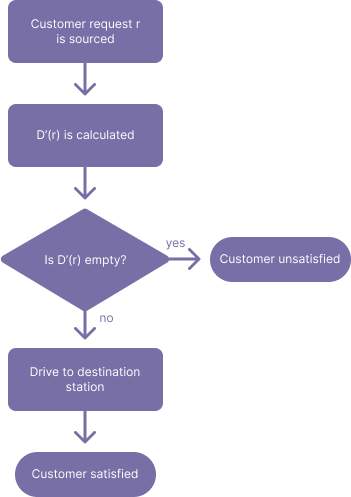
\includegraphics[width=.4\linewidth]{./Figures/event-flow.png}
  \caption{Simulation flow}
  \label{fig:Flow}
\end{figure}

The process that a typical customer request would flow through is given by Figure \ref{fig:Flow}. The flow is started by the
event that a customer request is sourced. This event happens periodically based on the average time period of demand $p_h$, determined
beforehand by existing demand data for each hour of the day $h \in [0,24) \subset \mathbb{N}$. The timestamp a customer request is registered with the system
is called $t_0$ from now on.

The customer then needs to make a vehicle decision based on the request $r$ and the current substitution effect
 $\alpha$ resulting in $D(r, \alpha)$. The framework then calculates a more restricted set of available
possible vehicle choices $D'(r, \alpha) = \{c \ |\ c \in D(r, \alpha) \land \Delta_{s_{r, 0}}(t_0, c) > -C\}$ which
includes the capacity restriction mentioned in Section \ref{sub_sec:Method/Concepts/Station}. If $D'$ is an empty set, the customer
request is labeled "unsatisfied" and $r$ is added to the set of unsatisfied requests $\mathbb{UR}$. Otherwise, a random unbiased choice between the classes in 
the set $D'$ is made resulting in the chosen class $c$ and the state of the start station is updated such that 
$$
\Delta_{s_{r, 0}}(t_0 + \epsilon, c) = \Delta_{s_{r, 0}}(t_0, c) - 1
$$
 
Following this the customer starts its rental and travels to $s_{r, 1}$. This takes him an amount of time $\delta t$ given by 
$\delta t = l_r / \text{AS}$ where $AS$ (average speed) is the average speed of urban commute. This customer then reaches
station $s_{r, 1}$ at time $t_1 = t_0 + \delta t$ and increases the delta function of the target station similarly to
$$
\Delta_{s_{r, 1}}(t_1 + \epsilon, c) = \Delta_{s_{r, 1}}(t_1, c) + 1
$$

The rental is then counted as complete, added to the set of satisfied requests $\mathbb{SR}$ and the total profit $\pi$ is increased by $\text{cost}(c, \delta t)$, completing the
customer request process. One run of the simulation framework simulates a whole day and includes the station network
as a shared resource.


\subsection{Metric \& Performance}
\label{sub_sec:Method/Metrics}

Resulting in performance metrics that can give measurable insights on the dynamics of the environment and
allows to analyze the effects of the models parameters such as the substitution effect $\alpha$ and the
capacity restriction $C$. The presented metrics aim to be of importance for operational decision-making
and connect the results of the simulation stage to real world performance of a car-sharing network.

\vspace*{4ex}
\renewcommand\tabularxcolumn[1]{m{#1}}
\renewcommand{\arraystretch}{1.6}
\begin{center}
\centering
\begin{tabularx}{0.9\linewidth}{@{}c|c|X@{}}
  \textbf{Metric} & \textbf{Defintion} & \textbf{Description} \\
  \hline
  URR & $\frac{|\mathbb{UR}|}{|\mathbb{UR}| + |\mathbb{SR}|}$ & The \textbf{U}nsatisfied \textbf{R}equest \textbf{R}atio, eg. the ratio of unsatisfied customers to all customers \\
  $\pi$ & {--} & The total profit of the simulation, calculated as part of the simulation stage \\
  TD & $\sum_{r \in \mathbb{SR}} l_r$ & The total distance driven during the day \\
\end{tabularx}
\end{center}

\renewcommand{\arraystretch}{1}



% Case Study
\clearpage
\section{Case Study Berlin SHARE NOW}
\label{sec:CaseStudy}

The methods described in Section \ref{sec:Method} are now applied to the specific case
of SHARE NOW in Berlin during a period between October 2019 and March 2020. Firstly
we will discuss SHARE NOW as a company and then later the dataset and the insights it
can deliver as well as the trained classifier and its application in the Simulation
environment we have described above. 

\subsection{SHARE NOW}

SHARE NOW is the worldwide leading free-floating car-sharing service.
As a free-floating service the user can pick up an available car anywhere in a defined zone
and finish the trip anywhere in that zone. It is currently available in 16 European cities
with 11000 vehicles, with nearly 3000 electric vehicles. With about 3.4 million customers
it has an unprecedented set of car-sharing users \cite{ShareNowAboutUs}. It was founded as 
part of a larger a joint venture of the BMW Group and the Daimler AG, which also includes
services like PARK NOW, CHARGE NOW, REACH NOW and FREE NOW. Both firms brought in their
existing car-sharing solutions, namely Car2Go a subsidiary of the Daimler AG and DriveNow
a subsidiary of the BMW Group into the joint venture. The merge led to an increase in ease of use for customers
while the venture parties could secure the leading market share at many of Europeans
largest car-sharing sites.


\subsection{Data sources}
\label{sub_sec:CaseStudy/Data}

This Case Study is primarily based on a dataset which includes 1.983.246 datapoints, each 
representing a trip made through SHARE NOWs service. Along other interesting fields each data point
contains the vehicle model of the rental, the location where the rental was started as well as the distance of the trip.
This data was then joined with publicly available socio-demographic data from Zensus 2011, a census
commissioned by the statistical federal office. 


\subsection{Fleet}
\label{sub_sec:CaseStudy/Fleet}

SHARE NOW uses an extensive fleet of vehicles for its car-sharing service according to their website. The data
for Berlin however indicates a slightly smaller set of available vehicles for that region. Throughout the
period of data collection a total of 3946 unique vehicles were tracked in the zone, with the following
distribution.

\begin{figure}[htbp]
  \centering
  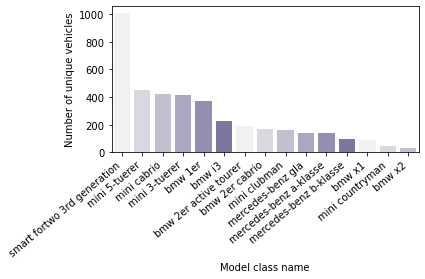
\includegraphics[width=.4\linewidth]{./Figures/fleet.png}
  \caption{Number of unique vehicles by class}
  \label{fig:Fleet}
\end{figure}

As can be seen in Figure \ref{fig:Fleet} the number of vehicles of each type is far from equally distributed.
The dominant model in terms of number of vehicles is by a large margin the smart fortwo with 1007 unique vehicles, 
offering a high value proposition
in terms of parking space and ease of use for urban commuting. A clear tendency towards smaller cars, such as smarts
or minis is visible in the distribution.

\begin{figure}[htbp]
  \centering
  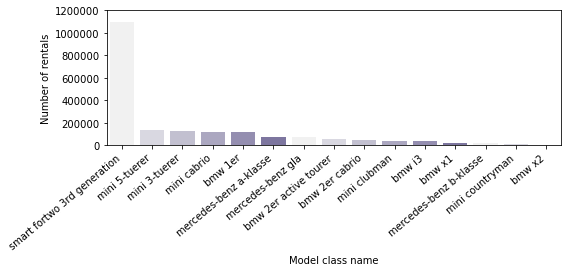
\includegraphics[width=.4\linewidth]{./Figures/travels.png}
  \caption{Number of rentals by class}
  \label{fig:Rentals}
\end{figure}

The actual amount of rentals, as shown in Figure \ref{fig:Rentals} has a very similar order to the fleet size 
with only a few exceptions. Notably though the smart has
seen even more demand than indicated by the number of vehicles.

The missing component however is the set of decidable classes. Similarly to the real world fleet deployment the
set of models is structured in terms of vehicle classes, namely $\mathbb{C} = \{ \text{XS}, \text{S}, \text{M}, \text{L} \}$.
Then each model was assigned to a class, the mapping can be found in Table \ref{table:VehicleClasses}.
These classes play an important role in the operational management of the car-sharing fleet since they differ in terms of costs and therefore profit.
 Additionally, we will define the cost function used in the simulation stage
of the framework based on the actual minute based pricing model of SHARE NOW. Although SHARE NOW also offers other tariffs we will focus one
the on-demand minute based charge system for this implementation \cite{ShareNowPricing}. The resulting function can be found in Table \ref{table:CostFunction}.

\subsection{Data preparation}
\label{sub_sec:CaseStudy/Preparation}

Before one could train the actual classifier the data had to be prepared to adhere to the form
required by the framework. Using the Zensus data an area description for each request was
build where the set of categories to be analyzed includes the age distribution as well as the martial status.
$\mathbb{X} = \{ \text{Age}, \text{Marital Status} \}$. Then ranges for each were defined as can be seen in Table \ref{table:Ranges}.
Subsequently rows with missing of malformed data were removed.

In early training iterations another important imbalance in the dataset was discovered. Classification models
trained on the data had a tendency to favor the "XS" class since there were far more rentals done with
vehicles from that class. To counteract that, since the set of features was missing an indicator for availability
of vehicles the data for each class was shuffled and truncated in such a way that
$\frac{nv(c_a)}{nv(c_b)} = \frac{nd(c_a)}{nd(c_b)} \ \forall c_a, c_b \in \mathbb{C}$, where $nv: \mathbb{C} \to \mathbb{N}$ is a function
that returns the number of vehicles of a specific category and $nd: \mathbb{C} \to \mathbb{N}$ is a function that returns the
amount of datapoints in the training set for each category. Reducing the impact of the availability of vehicles for
the classification task.

\subsection{Classifier}
\label{sub_sec:CaseStudy/Classifier}

Resulting in a dataset that mapped the framework definition of the customer request onto the class that the customer choose.
That data was then normalized into a zero to one range and split into a
training and a testing set and a Complement Naive Bayes classifier (CNB) was fit using
the training data. A Complement Naive Bayes Classifier is an adaption of a Multinomial Naive Bayes classifier, most
prominently known from text classification tasks. Additionally, the CNB typically has an advantage when dealing
with imbalanced dataset such as ours \cite{rennie2003tackling}.


\subsection{Simulation}
\label{sub_sec:CaseStudy/Simulation}

\begin{figure}[htbp]
  \centering
  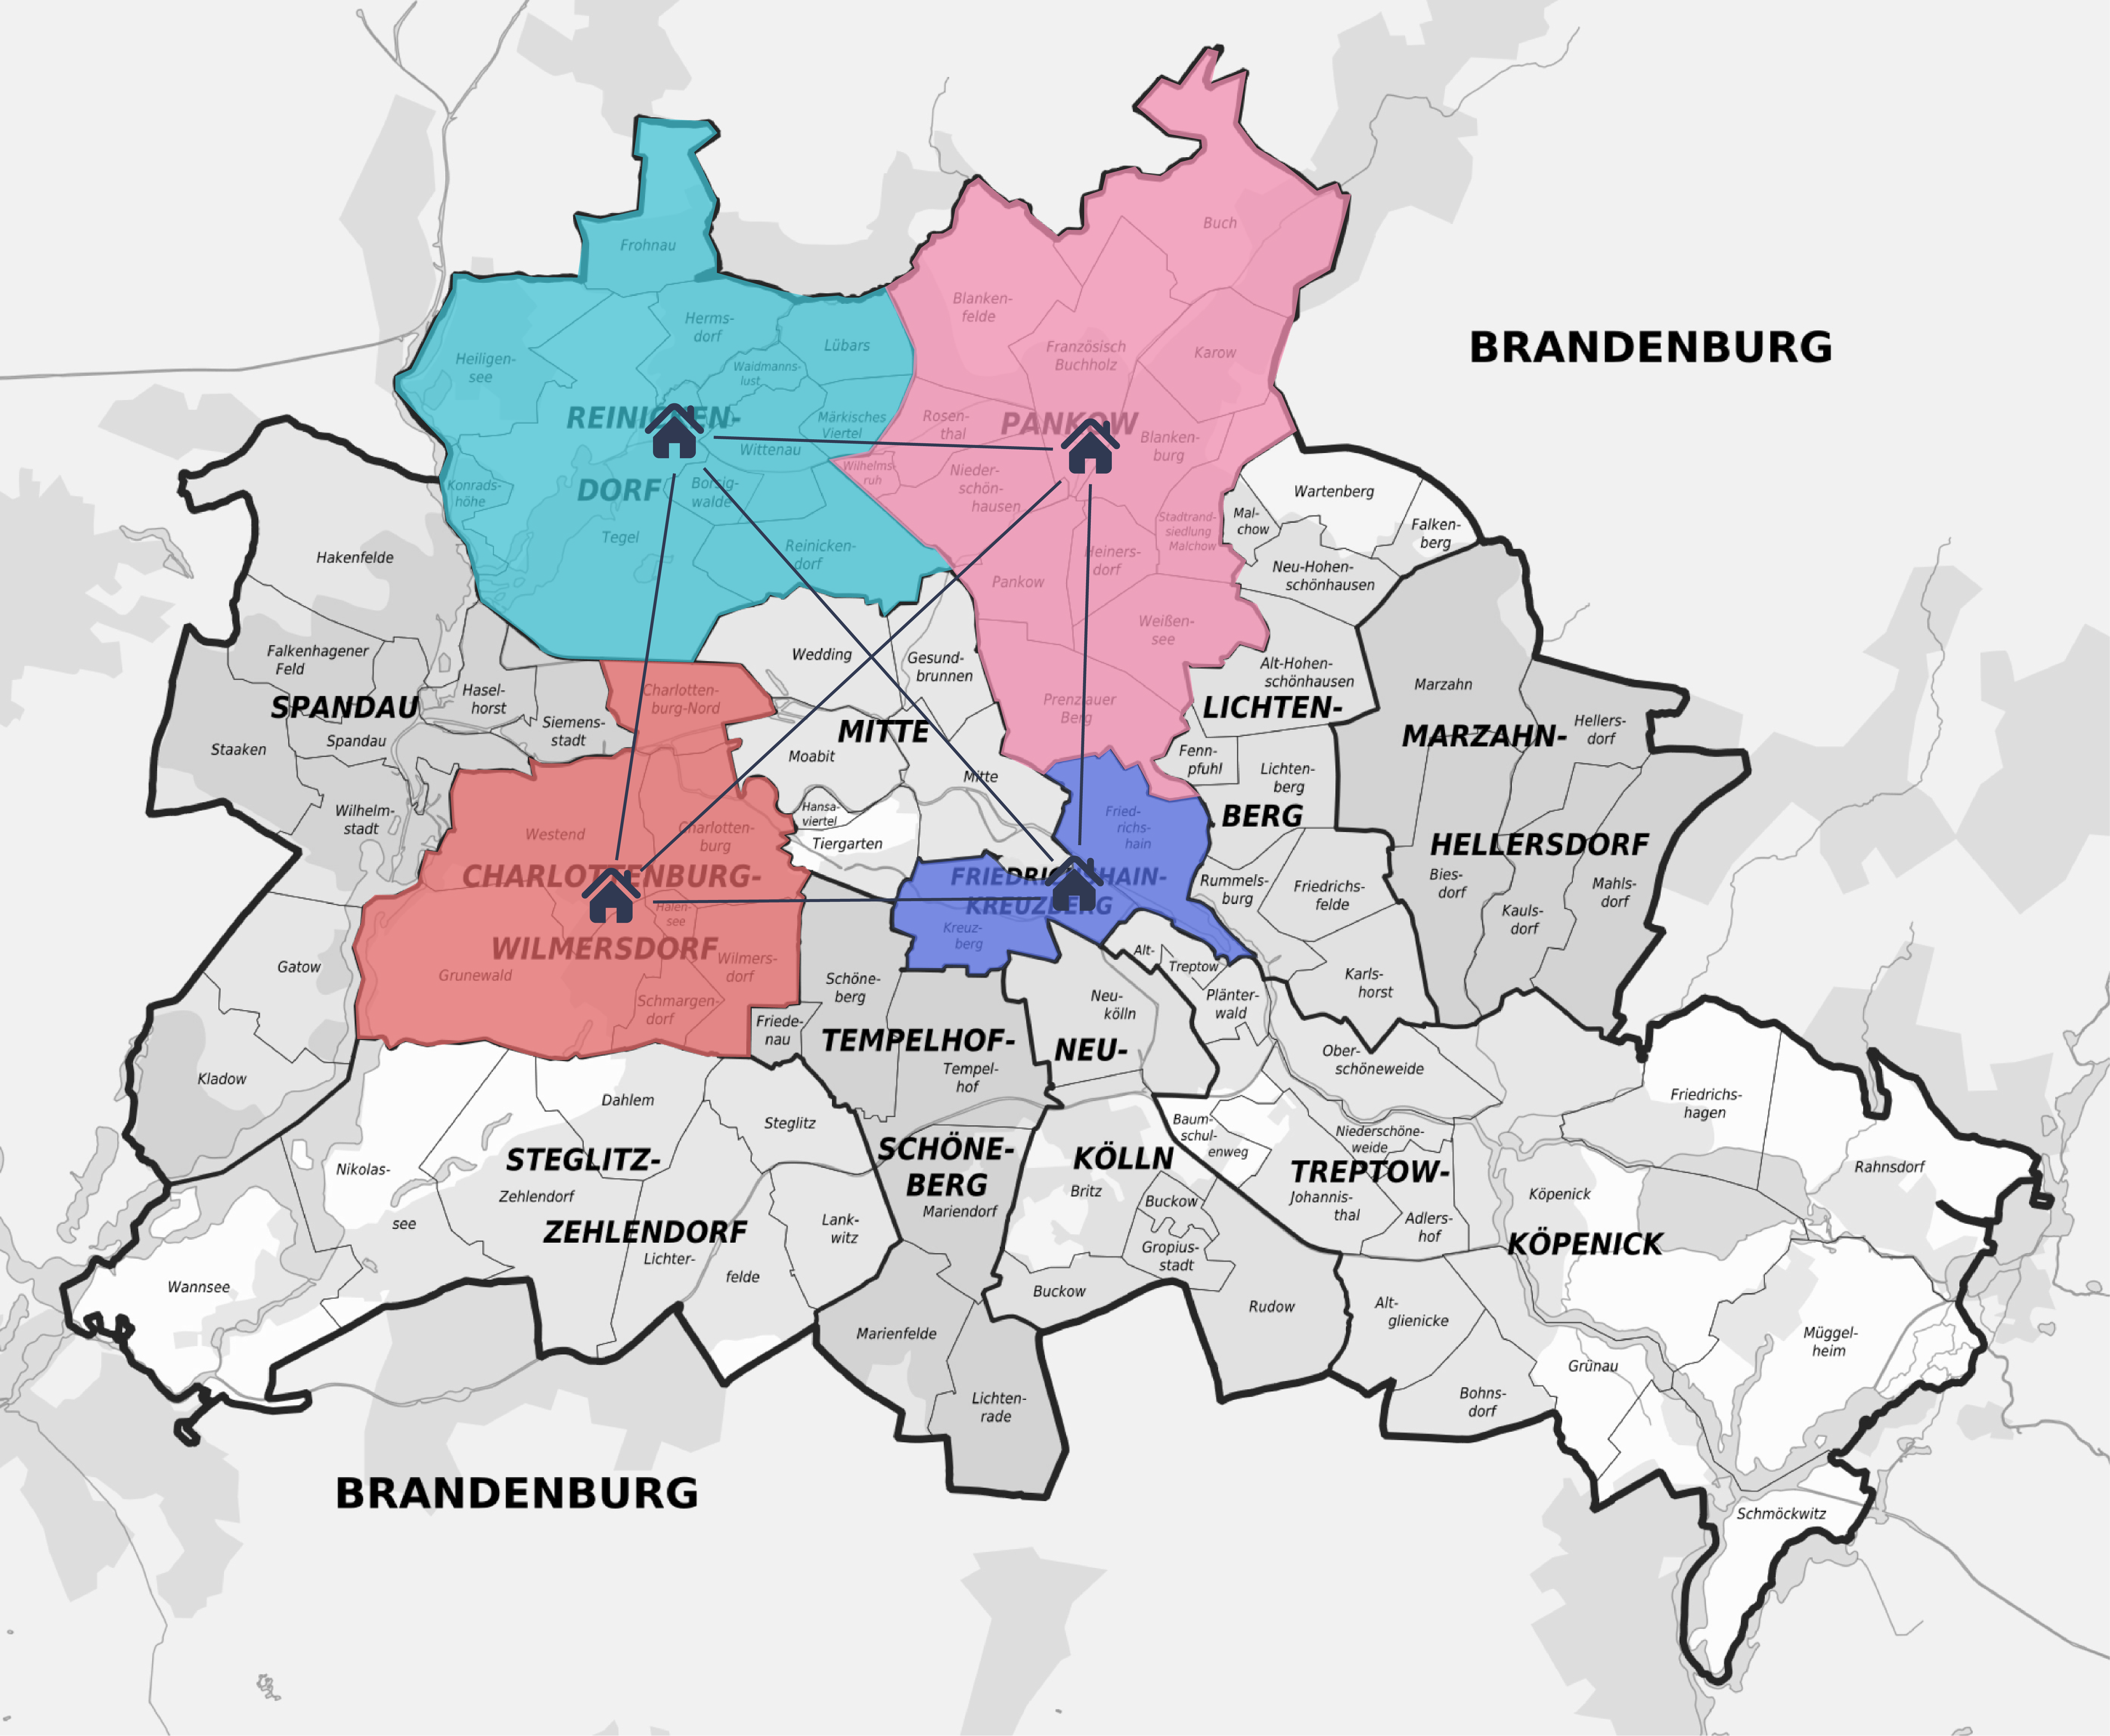
\includegraphics[width=.5\linewidth]{./Figures/graph.png}
  \caption{Simulation Graph}
  \label{fig:Graph}
\end{figure}
Before the actual implementation of the simulation stage, some data had to be prepared. Firstly 
the set of stations was to be defined, setting up the real world context of the simulation 
framework. Since the data was sourced in the city of Berlin, the simulation will also take place
in that setting. Firstly the area data regarding the age and marital status where sourced for various
districts in Berlin, as can be seen in Table \ref{table:Districts}. Then a subset of these were selected
to contain stations of our proposed simulation framework. This then forms our simulation graph as can be
seen in Figure \ref{fig:Graph}.


Afterwards the distance function $L: \mathbb{E} \to \mathbb{R}$ was determined for each edge in the proposed graph and can be found
in Table \ref{table:Distance}. Using this we can define the set of stations $\mathbb{S} = \{ \text{Pankow}, \text{Reinickendorf}, \text{Kreuzberg}, \text{Charlottenburg} \}$,
where the area function is the identity function. Concluding the definition of the setting of the simulation.

\begin{figure}[htbp]
  \centering
  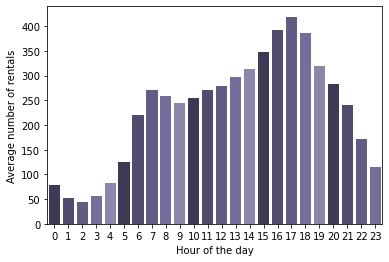
\includegraphics[width=.5\linewidth]{./Figures/hourly-demand.png}
  \caption{Average hourly demand of selected districts}
  \label{fig:Demand}
\end{figure}

Secondly, the simulation stage also requires the average time-period between customer arrivals for each working hour.
This was computed based on the dataset, by extracting datapoints which happened in the simulation areas $\mathbb{S}$ 
and grouping into days and then taking the average for each hour. The resulting
demand distribution can be seen in Figure \ref{fig:Demand}. The time period $p_h \ \forall h \in [0, 34] \subset \mathbb{N}$
can then be determined by $p_h = \frac{1}{\text{demand}_h}$ where $\text{demand}_h$ are the values from the figure.
Additionally, the value of $AS$ the average speed of urban commute was determined from the dataset to be $AS = 126.39 \frac{\text{m}}{\text{min}}$.

Using this information and the classifier described in Section \ref{sub_sec:CaseStudy/Classifier}, the simulation environment
was build in Python 3.10 using the SimPy library. The simulation receives the parameters $\alpha, C$ (Substitution Effect, Capacity),
the set of stations to be simulated, the hourly demand as well as the predictor function. That way different kind of classifiers
could be trained to quickly assess the performance of different classification models. The implementation
is also available as part of the publicly available accompanying GitHub repository.

% Simulation
% \clearpage
\section{Simulation}
\label{sec:Simulation}

\subsection{Model Restrictions}
\label{subsec:Simulation/restrictions}


% Vehicle Choice Model
% \clearpage
\section{Vehicle Choice Model}
\label{sec:ChoiceModel}

Mathematical description of vehicle choice model

% Maybe a model that calculates if a vehicle will be rented
Palette: https://flatuicolors.com/palette/ru


\subsection{Data source}
\label{sub_sec:DataSource}

- Dataset 4gb
- Zensus data


\subsection{Data preparation}
\label{sub_sec:DataPreparation}

- Huge bias towards smart fourtwo
- Missing income
- 


\begin{itemize}
  \item House hold -> Size relation
  \item College to size -> No real thingy
  % \item Dataset: https://www.kaggle.com/steventaylor11/stated-preferences-for-car-choice
\end{itemize}

Features:

We propose a person, which is defined by a feature vector. From now on a person strictly refers to a specific realization 
of these features unless mentioned otherwise. 

\begin{longtable}{l | c}
  \caption{Features}
  \label{table:features}
  \\
  \textbf{Label} & \textbf{Description} \\
  \hline
  age & The current age of this person, must be > 18 years. unbounded otherwise \\
  hss & Household size\\
  college & 1 (or true) if the person had college education, 0 (or false) otherwise \\
  income & Monthly income, before taxes \\
  comm & Commuting distance (daily)
\end{longtable}

Scoring algorithm with the following "decisions":

Early opt out case: $age < 21$: Typically only the XS category is allowed to be driven by persons under the age of 21.
Otherwise we will employ a scoring algorithm which, where we calculate a score $s(o)$ where 
$o \in \{ \textrm{XS}, \textrm{S}, \textrm{M}, \textrm{L} \} = C$. The score is based on various sub-scores, namely:
$$
s_0(o) = 
\begin{cases}
  1 - P(\text{hss} > 2 \land \text{category} = o), & \text{if}\ \text{hss}\ \le 2 \\
  P(\text{hss} > 2 \land \text{category} = o), & \text{otherwise}
\end{cases}
$$
where $P(\text{hss} > 2 \land \text{category} = o) \ \forall o \in C$ is determined empirically by using the data source 
mentioned in \ref{sub_sec:DataSource} and can be found in the Appendix\todo{Add that to the Appendix}. Another important 
scoring mechanism depictures a correlation between commuting distance and the size an can be similarily described as:
$$
s_1(o) = 
\begin{cases}
  1 - P(\text{comm} > 2 \land \text{category} = o), & \text{if}\ \text{hss}\ \le 2 \\
  P(\text{comm} > 2 \land \text{category} = o), & \text{otherwise}
\end{cases}
$$



% Results & Discussion
\clearpage
\section{Results \& Discussion}
\label{sec:Results}


Succeeding the implementation phase the results of the simulation framework had to be analyzed. Due
to the complexity and high dimensionality of the problem, a focus was made on the effects of the parameters
$C$ and $\alpha$ on the metrics defined in section \ref{sub_sec:Method/Metrics}.

\subsection{Simulation Result}
\label{sub_sec:Results/Results}

\begin{figure}[htbp]
  \centering
  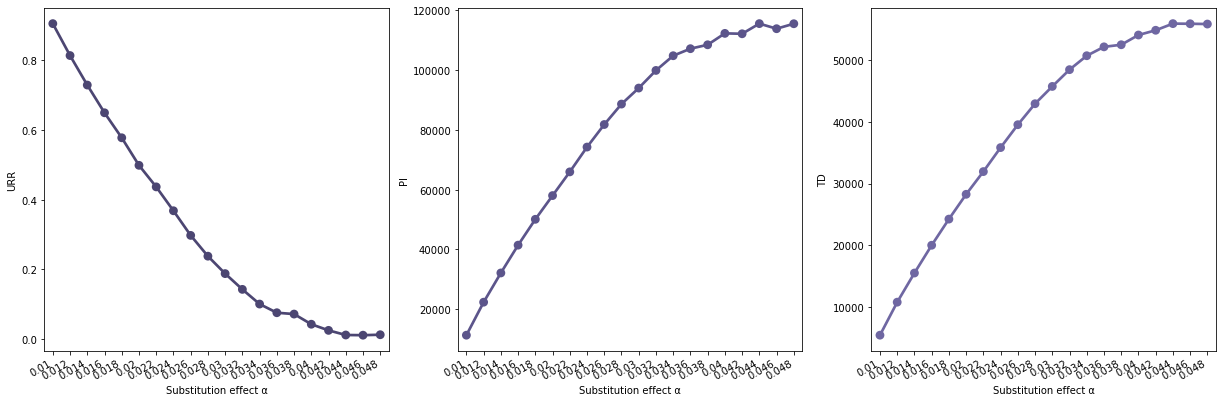
\includegraphics[width=\linewidth]{./Figures/alpha.png}
  \caption{Effects of alpha for performance metrics}
  \label{fig:Alpha}
\end{figure}

Starting with the effect of the substitution effect $\alpha$. The Figure \ref{fig:Alpha} shows the
metrics defined in Section \ref{sub_sec:Method/Metrics} in order. For this evaluation the capacity
was set to $C = 5$, leading to a higher importance of the substitution effect. A clear dependency
of the value of alpha to a higher performing car-sharing network can be seen. However, the curves
also indicate that the impact of the parameter decreases with larger values and the random
signal, that is due to the random nature of the simulation environment, increases.

\begin{figure}[htbp]
  \centering
  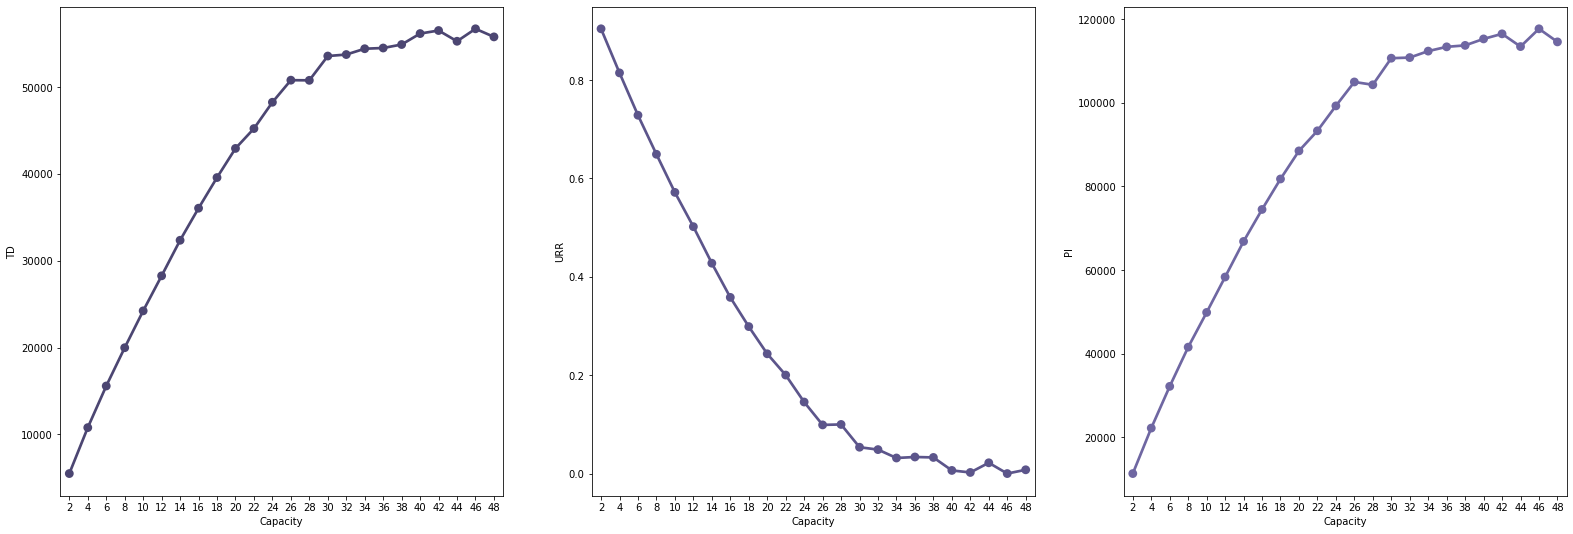
\includegraphics[width=\linewidth]{./Figures/capacity.png}
  \caption{Effects of capacity for performance metrics}
  \label{fig:Capacity}
\end{figure}

A very similar effect can be seen in Figure \ref{fig:Capacity} with the parameter $C$,
the capacity at each station. For these the alpha value has been set to $\alpha = 0.05$,
the optimal value based on previous results. From an operational standpoint an optimal
fleet capacity could be determined by averaging the metrics over multiple runs
and define a threshold below which the increase in overall performance with regard to the
increase in fleet size provides no added value to the network. This effect was also discovered
by \shortciteA{Nourinejad2014}.

\begin{figure}[htbp]
  \centering
  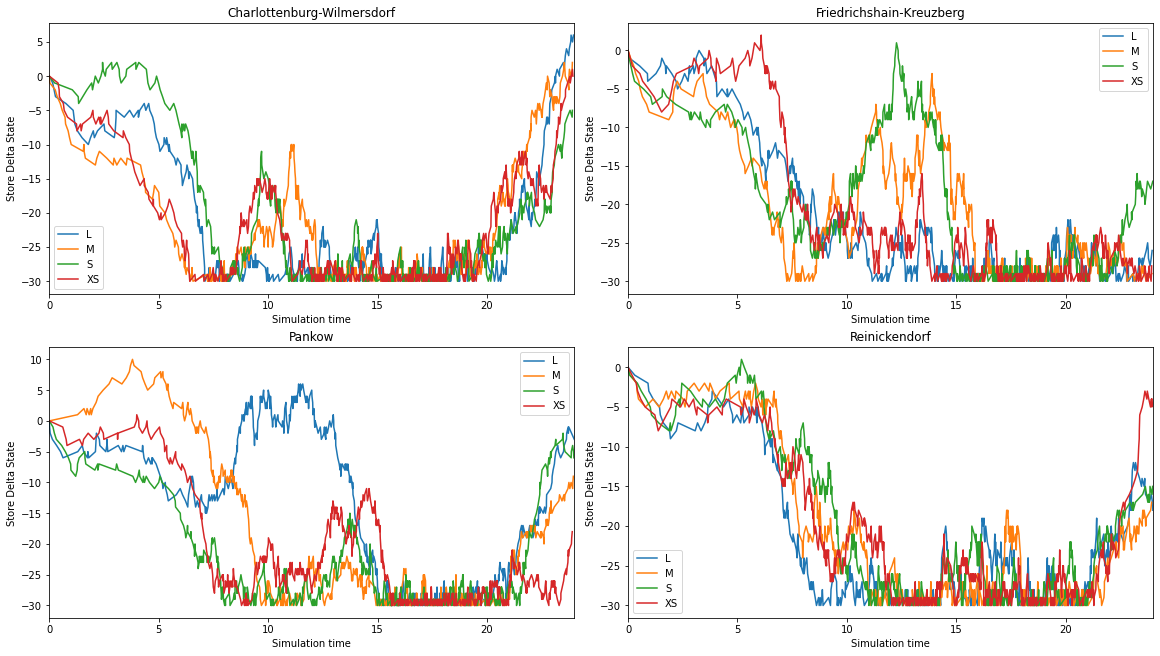
\includegraphics[width=\linewidth]{./Figures/delta-func.png}
  \caption{$\Delta_s(t, c)$ for a simulation with $\alpha=0.003, C=30$}
  \label{fig:DeltaFunc}
\end{figure}

Lastly the state function of the stations $\Delta_s(t, c)$ has been plotted against the
simulation time, to get insights of the state at each station throughout the working day.
As can be seen in Figure \ref{fig:DeltaFunc}, the impact of the demand described in Figure \ref{fig:Demand}
is clearly visible. Especially during the rush hour in the late afternoon all stations
reach capacity limits, but just about manage to keep up with an unsatisfied customer rate (URR)
of just 6.50\%. 

\subsection{Discussion \& Further Research}
\label{sub_sec:Results/Discussion}

As mentioned previously the topic of simulation in a large scale network, like a car-sharing network,
is a problem with high-dimensionality, therefore providing a lot of potential further research areas.
The focus of this thesis also included to make the simulation environment as general 
as possible, such that additional research could be conducted on the same code base.

One aspect that could be of interest, is the selection of start and end stations for
each customer request. In the real world this is typically not equally distributed but
often follows traffic flows, which are among others time and location dependent.
Another potential extension, could include an increased set of stations $\mathbb{S}$ to
study even larger car-sharing networks.

While training the classifier, it became apparent that the signal of the socio-demographic
data of the rental area only correlated loosely with the decision made, and feature importance
was quite low. In further research a more sophisticated classifier could be trained that
sources a dataset which directly correlates one rental to for example the age of the
customer. Due to the modularity of the simulation that model could then easily be
exchanged with the classifier trained in this thesis and used in the simulation 
environment. 

Another aspect that would be of particular interest for the simulation stage is the parameter
$\alpha$. This parameter is not controllable by the operator but inherent for a particular
customer group. One could convey a study to try to estimate the real world $\alpha$ for different
deployments of a car-sharing networks empirically.


% Conclusion
\clearpage
\section{Conclusion \& Further Research}
\label{sec:Conclusion}

\subsection{Exemplary Citation}
\label{subsec:Section_Name_X/cite}

% use \shortciteA when using author names in text

In this research we follow \shortciteA{Ketter2016}...

% use \shortcite to reference normally in brackets

PowerTAC is an example of a multiagent competitive gaming platform \shortcite{Ketter2016}.

%%%%%%%%%%%%%%%%%%%%%%%%%%%%%%%%%%%%%%%%%%%%%%%%%%%%%%%%%%%%%
%APPENDICES
%%%%%%%%%%%%%%%%%%%%%%%%%%%%%%%%%%%%%%%%%%%%%%%%%%%%%%%%%%%%%


\appendix
\renewcommand*{\thesection}{\Alph{section}}\textbf{}

% APPENDIX A
\clearpage
\section{Appendix}
\label{app:A}
...

%%%%%%%%%%%%%%%%%%%%%%%%%%%%%%%%%%%%%%%%%%%%%%%%%%%%%%%%%%%%%
%BIBLIOGRAPHY
%%%%%%%%%%%%%%%%%%%%%%%%%%%%%%%%%%%%%%%%%%%%%%%%%%%%%%%%%%%%%

\clearpage
\renewcommand*{\thesection}{}\textbf{}

\bibliographystyle{apacite}
\bibliography{Bibliography.bib}


\end{document}
